%%% Copyright 2004 by Till Tantau <tantau@users.sourceforge.net>.
%%% Modified by Ken Wilder. Modified again by Winnie van Dijk.
%%% The original can be found in the beamer distribution.

\documentclass{beamer}

%%% Set the theme
\usepackage{style/wvd_beamertheme_lecture}


%%% View lists in a stepwise fashion, not all at once
%\beamerdefaultoverlayspecification{<+->}




%%% Define the title page elements
\title
	{Introduction to R for Economists}
\subtitle[Part 2]
	{Basic Programming Principles and Data Analysis (Part 2)
	}
\setcounter{lecture}{2} %This sets the counters for theorems, examples, etc.
% \author{}
% \institute[University of Chicago]
	% {University of Chicago / Becker Friedman Institute}






\begin{document}

%%% Title frame
\begin{frame}
  \titlepage
\end{frame}

\note{notes}

%%% Outline frame
\begin{frame}[allowframebreaks]
 \frametitle{Outline}
 \tableofcontents%[pausesections]
\end{frame}

\note{notes}




% INTENDED OUTLINE

%Part 1: Intro to R, Matlab \& LaTeX
%1.    Good programming practice
%2.    Recap of R
%3.    Intro to Matlab (mostly comparing Matlab syntax to R)
%4.    Latex (based on https://www.sharelatex.com/learn/Learn_LaTeX_in_30_minutes)

%Part 2: Selected topics in economic data with illustrations in R
%5.    Functional approximation (to illustrate optimization and plotting using ggplot)
%6.    Census data / APIs
%7.    Useful public data sets
%8.    Making maps with ggmap
%9.    Useful packages (maybe also creating your own packages)
%10.   Summarizing data using data.tables and the tidyverse 
%11.   Ggplot examples (cheat sheet)
%12.   Packages
%13.   Shiny
%14.   Knitr and R notebooks
%15.   Git and Github









%%% Main content

\section{Intro \& logistics}

\begin{frame}[allowframebreaks]
 \frametitle{Administration}

	\begin{itemize}
	\setlength{\itemsep}{\fill}
		\item
		Today's workshop:
		\begin{itemize}
			\item
			Part 1 (morning): Good programming practice, introduction to R and Matlab.
			\item
			Part 2 (afternoon): Selected topics for data analysis in R.
		\end{itemize}
		\vfill
		\item
		Part 2 learning objectives: 
		\begin{itemize}
		    \item
		    Useful data sources: IPUMS, Web APIs
		    \item
		    Importing data: Census API, \textts{foreign} package
		    \item
		    Shaping data: \textts{data.tables} %\textts{data.frames} and \textts{dplyr}, 
		    \item
		    Describing data: \textts{ggplot2} and \textts{ggmap} packages
		    \item
		    Quick overview of methods for reporting on your results (R Notebooks, knitr, Shiny)
		    \item
		    Some useful packages, why and how to build your own package
		\end{itemize}
		\vfill
		\item
		Required software:
		\begin{columns}[t]
		\begin{column}{0.1\textwidth}
		\end{column}
		\begin{column}{0.8\textwidth}
		\begin{itemize}
			\item[R and RStudio]
			\vskip-.5cm
			Can be downloaded free of charge from \scriptsize\url{http://www.rstudio.com/}\small.
			%\item[LaTeX editor]
			%\vskip-.2cm
			%Texmaker is recommended. I don't mind if you use ShareLaTeX or LyX, but some things I show you today will not work with those editors. You can download Texmaker from \scriptsize\url{http://www.xm1math.net/texmaker/}\normalsize.
			\vfill
		\end{itemize}
		\end{column}
		\end{columns}
		\vfill
		\item
		I will show you example code, switching between slides and RStudio. We will go slowly, so that you can follow along on your own laptops.
		\vskip.2cm
		\begin{itemize}
			\item
			Commands from demonstrations are in the file \textts{REU\_commands.R} on the website.
			\item
			Solutions to exercises are also in that file.
		    \vfill
		\end{itemize}
		\vfill
		\item
		Afterwards, I will distribute these slides, along with example code and practice problems that you can try at home.
		\vfill
		\item
		There's a list of additional resources at the end of this slide deck, in case you want to learn more.
		\vfill
		\item
		If you have suggestions on how to improve this workshop, you can always email me. Your feedback is highly appreciated!
	\end{itemize}

\end{frame}



\section{Useful data sources}

%\subsection{IPUMS}

\begin{frame}[allowframebreaks]
 \frametitle{IPUMS}

	\begin{itemize}
	    \item
	    IPUMS = Integrated Public Use Microdata Series.
	    \vskip.4cm
        \item
        IPUMS description: \textit{``provides census and survey data from around the world integrated across time and space. IPUMS integration and documentation makes it easy to study change, conduct comparative research, merge information across data types, and analyze individuals within family and community context. Data and services available free of charge.''}
	    \vskip.4cm
        \item
        It's an easy way to obtain survey data from the Census, CPS, ATUS, ACS, and more.
	    \vskip.4cm
		\item
		You can access IPUMS here: \scriptsize\url{https://www.ipums.org/}\normalsize .
		\vskip5cm
	\end{itemize}
	
	To use IPUMS:
    \begin{enumerate}
	    \item 
	    Go to the IPUMS website. You will see an overview of all the surveys they offer.
	    \item 
	    Select the data source you're interested in. Let's say you want to use IPUMS USA (Census microdata).
	    \item 
	    At the top of the page you will see the option to log in, click that.
	    \item 
	    On the Login page you will see a button to create new account. Go ahead and do so.
	    \item 
	    After you create an account you can get data here: \scriptsize\url{https://usa.ipums.org/usa-action/variables/group}\normalsize. Click ``select samples'' to pick the years of data you want, and click the variables you want from the drop-down menus or using the search option.
	    \item 
	    When you are done, check out your datacart! (Ask IPUMS to give you a \textts{.csv} file during checkout)
	    \vskip5cm
    \end{enumerate}
	
	Advantages of using IPUMS:
	\begin{itemize}
	    \item 
	    Harmonized variables! Surveys may slightly change format over the years (e.g., questions asked or spatial definitions in the ACS), and so you would have to clean your data to make everything fit together. IPUMS does this for you.
	    \item 
	    Easy to select variables and samples
	    \item
	    Automatically generated data documentation.
    	\item 
    	Easy to update your data set by editing past sample selection settings associated with your account.
    	\item
    	Great support staff.
    	\item
    	IPUMS includes:
    	\begin{itemize}
    	    \item
    	    CPS (Current Population Survey) microdata
    	    \item
    	    NHGIS: Census and ACS data combined with with GIS-compatible boundary files
    	    \item
    	    American Time Use Survey
    	    \item
    	    Census microdata from 81 other countries
    	    \item
    	    Lots of other stuff to explore
    	\end{itemize}
	\end{itemize}
	
	\vskip5cm
	
	\begin{myexc}[Using IPUMS/NHGIS]
	\fontsize{10pt}{12}\selectfont
        \begin{enumerate}[(a)]
	        \item
	        Use the NHGIS section of IPUMS to find county-level per-capita income data from the 2013 ACS. The variable you are looking for is\\
	        \textts{B19301. Per Capita Income in the Past 12 Months (in 2013 Inflation-Adjusted Dollars)}.
	        \item
	        Add this variable to your data cart and download it in .csv format.
	        \item
	        Save the file in a convenient folder.
        \end{enumerate}
    If this didn't work, you can download the file \textts{NHGIS0009\_DS199\_2013\_COUNTY.csv} from \href{https://sites.google.com/site/reu2017vandijk/data}{\textts{\scriptsize http://sites.google.com/site/reu2017vandijk/data}}. The file \textts{
NHGIS0009\_DS199\_2013\_COUNTY\_CODEBOOK.txt} is the codebook that should have come with your NHGIS download. It contains descriptions of the variables you selected.
	\addtocounter{exccounter}{1}
	\end{myexc}
	
\end{frame}



\section{Importing data}

\subsection{Importing saved data files}

\begin{frame}%[allowframebreaks]
 \frametitle{Importing saved data files}
 	
 	\begin{itemize}
 	    \item 
 	    For ``simple'' rectangular files like \textts{.csv} and \textts{.txt}, use the \textts{readr} package. This reads in data much faster than base R.
 	    \item 
 	    If you have foreign files like \textts{.dta} files (from Stata) or \textts{.sav} files (from SPSS), you can use the \textts{haven} package, which can handle up to Stata 14.
 	    \item
 	    The \textts{readxl} package is useful for reading in Excel files.
 	    \item 
 	    For large files, the function \textts{fread} from the \textts{data.table} package can be useful.
 	    \item
 	    For previously saved R objects (with extension \textts{.RData}), use the base function \textts{load()}.
 	    \vfill
 	\end{itemize}
	
	\begin{myexc}[ACS data]
	\fontsize{10pt}{13}\selectfont
	    Set your working directory to the folder where you previously saved the ACS data, and read it into R. Save the object R creates under the name \textts{county\_data}.
	    \begin{itemize}
	        \item
	        To use a package, you need to first install and then load it:
	        \scriptsize
            \begin{verbatim}
            
            install.packages(<package name>)
            
            library(<package name>)
            \end{verbatim}
	    \end{itemize}
	\addtocounter{exccounter}{1}
	\end{myexc}
	
\end{frame}




\subsection{Web APIs}

\begin{frame}[allowframebreaks]
 \frametitle{Web APIs}

	\begin{itemize}
	    \item
	    API = application programming interface.
	    \vfill
	    \item
	    There are packages available that let you communicate with an API to import data.
	    \begin{itemize}
	        \item
	        Such a package provides methods that allow you to specify a URL, and the information in that location is automatically interpreted by R.
	        \vfill
	    \end{itemize}
	    \item
	    For example:
	    \begin{itemize}
	        \item
	        The \textts{rtimes} package lets you import data from a number of different APIs maintained by the New York Times: \scriptsize\url{https://cran.r-project.org/web/packages/rtimes/vignettes/rtimes_vignette.html}\small
	        \item
	        The \textts{OECD} can be used to import data from the OECD API: \scriptsize\url{https://cran.r-project.org/web/packages/OECD/OECD.pdf}\small
	        \item
	        OpenStreetMap and Google Maps API (\textts{RgoogleMaps})
	        \item
	        The \textts{RFacebook} packages allows you to analyze your own or public Facebook posts
	        \item
	        \textts{UbeR} to analyze your own Uber data
	        \vfill
	    \end{itemize}
	    \vskip-1.4cm
	    \item
	    In the next example we'll use the Census API to obtain the county-level income data from the ACS.
	\end{itemize}

	\begin{myexc}[The Census API]
	\fontsize{9pt}{11}\selectfont
        \begin{enumerate}[(a)]
	        \item
	        Go to \textts{\url{http://api.census.gov/data/key\_signup.html}} and request a US Census API key. You will get an email with the key, which you need to activate.
	        \item
        	Install and load the \textts{acs}, \textts{choroplethr}, \textts{choroplethrMaps}, and \textts{ggplot2} packages (make sure you have the more recent version of ggplot2). Then type \textts{api.key.install("<your key>")} into the command line, copy-pasting your personal key.
        	\item
        	Obtain 2013 county-level demographics and save them in a dataframe by typing\\
        	\textts{mydata <- get\_county\_demographics(2013)}. To get a sense of what the data looks like, you can view the first entries of the dataframe with the command \textts{head(mydata)}.
        	\item
        	Save a new dataframe object that conforms to the requirements of the plotting command in the next step:\\
        	\textts{df <- data.frame(region=mydata\$region,value=mydata\$per\_capita\_income)}.
        	\item
        	Plot:
        	\textts{county\_choropleth(df, title="County-level per capita income, 2013")}.
        \end{enumerate}
        %Note: Steps (iv)-(vi) could have been executed all at once using the command \textts{county\_choropleth\_acs}.
	\addtocounter{exccounter}{1}
	\end{myexc}
	
    If using the API didn't work, you can download the file \textts{county\_data.csv} from \href{https://sites.google.com/site/reu2017vandijk/data}{\textts{\scriptsize http://sites.google.com/site/reu2017vandijk/data}}.
	
	\begin{figure}
	\centering
	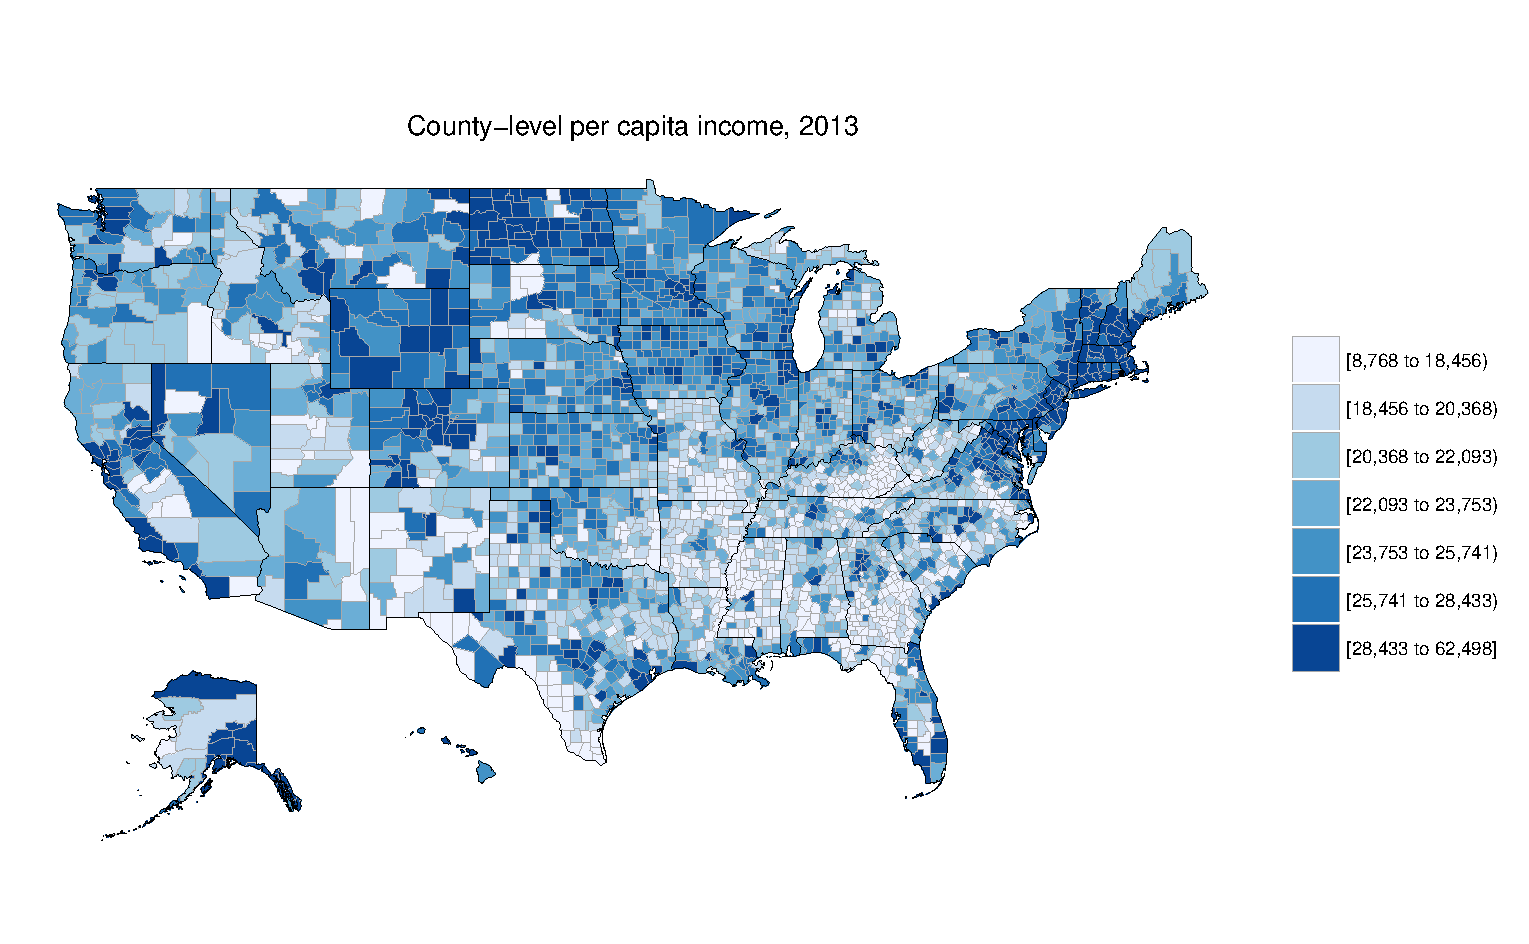
\includegraphics[width=0.7\textwidth]{figures/R_plot_map}
	\caption{\scriptsize County per capita income.}
	\label{Fig: map}
	\end{figure}
	
\end{frame}






\section{Storing and manipulating data}

\begin{frame}%[allowframebreaks]
 \frametitle{Object types for storing and manipulating data sets}
 
 	\begin{itemize}
 	    \item
 	    Two object types for storing data sets in R are \textts{data.frame} and \textts{data.table}.
 	    \vskip.5cm
 	    \item
 	    They come with their own syntax for manipulating data: \textts{dplyr} is great for \textts{data.frame}, and \textts{data.table} has its own syntax.
 	    \vskip.5cm
 	    \item
 	    \textts{data.table}  is  better  for  big  data. Because of this, if you are new to R, you should probably focus on learning \textts{data.table}.
 	\end{itemize}

\end{frame}


\subsection{The \small\texttt{data.frame} \normalsize and \small\texttt{dplyr} \normalsize packages}

\begin{frame}%[allowframebreaks]
 \frametitle{\texttt{data.frame } and \texttt{ dplyr}}
 
	\begin{myexc}[ChickWeight, data.frame]
	\fontsize{9pt}{11}\selectfont
        \begin{enumerate}[(a)]
	        \item
	        Download and attach the \textts{datasets} package. The \textts{ChickWeight} data frame has data from an experiment on the effect of diet on early growth of chicks. To load it as a \textts{data.frame}:\\
	        \textts{df <- data.frame(ChickWeight)}.
	        \item
	        Inspect the structure of the data set, for example using the command \textts{head()}, or the command \textts{describe()} in the \textts{Hmisc} package.
	        \item
	        Load the \textts{dplyr} package. What are the results of the following commands?
	        \begin{enumerate}[(i)]
	            \item
	            \textts{df\$Diet}
	            \item
	            \textts{df[df\$Diet == 1, ]}
	            \item
	            \textts{df\$Chick[df\$Diet == 1]}
	            \item
	            \textts{df2 <- df \%>\% group\_by(Chick)  \%>\% summarise(weight\_gain = max(weight) - min(weight), diet = Diet[1])}
	            \item
	            \textts{df2 \%>\%  group\_by(diet) \%>\% summarise(mean\_weight\_gain = mean(weight\_gain), 
sd\_weight\_gain = sd(weight\_gain))}
	        \end{enumerate}
        \end{enumerate}
        
	\addtocounter{exccounter}{1}
	\end{myexc}
 
\end{frame}




\subsection{The \small\texttt{data.table} \normalsize package}

\begin{frame}%[allowframebreaks]
 \frametitle{\texttt{data.table}}
 
	\begin{myexc}[ChickWeight, data.table]
	\fontsize{9pt}{11}\selectfont
        \begin{enumerate}[(a)]
	        \item
	        Return to the \textts{ChickWeight} example from Exercise 2.4, but now create a \textts{data.table}:\\
	        \textts{dt <- data.table(ChickWeight)}.
	        \item
	        What are the results of the following commands?
	        \begin{enumerate}[(i)]
	            \item
	            \textts{dt[Diet == 1, ]}
	            \item
	            \textts{dt[Diet == 1, list(Time,Chick)]}
	            \item
	            \textts{dt[Diet == 1, .(Time,Chick)]}
	            \item
	            \textts{dt[ , .(.N), by = Diet]} {\color{beamer@myRed} $\leftarrow$ you'll need this command again soon}
	            \item
	            \textts{dt2 <- dt[, list(weight\_gain = max(weight) - min(weight), diet = Diet[1]), by = Chick]}
	            \item
	            \textts{dt2[, list(mean\_weight\_gain = mean(weight\_gain), sd\_weight\_gain = sd(weight\_gain)), by=list(diet)] }
	        \end{enumerate}
	        \item
	        What is the variation in weight on day 2 of the study? %What is the variation in weight on day 2, by diet?
        \end{enumerate}
        
	\addtocounter{exccounter}{1}
	\end{myexc}
 
\end{frame}






\section{Visualizing data}

\subsection*{Describing data}

\subsection{The \small\texttt{ggplot2} \normalsize package}

\begin{frame}[allowframebreaks]
 \frametitle{The \Large\texttt{ggplot2} package}
 
		\vskip-.4cm
	\begin{myexc}[The Daily Show]
	\fontsize{10pt}{12}\selectfont
	\small In this exercise we'll reproduce the graph in this article: \scriptsize\url{https://fivethirtyeight.com/datalab/every-guest-jon-stewart-ever-had-on-the-daily-show/}\small.
        \begin{enumerate}[(a)]
	        \item
	        FiveThirtyEight has a package that allows us to import the data: \textts{fivethirtyeight}. We will also use the \small\textts{ggthemes} package to recreate the style. Please install these two packages.
        \end{enumerate}
        
	%\addtocounter{exccounter}{1}
	\end{myexc}

		\vskip-.5cm
		\begin{figure}
		\centering
		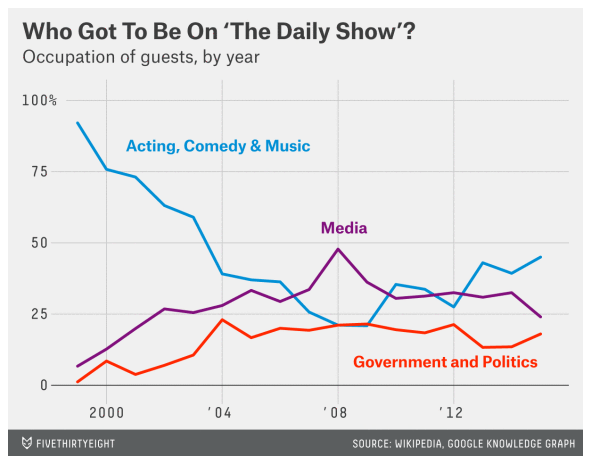
\includegraphics[width=.43\textwidth]{figures/dailyshow}
		\caption{\scriptsize Taken from the August 6, 2015 FiveThirtyEight article ``Every Guest Jon Stewart Ever Had On The Daily Show''.}
		\label{Fig: 1}
		\end{figure}
	
	\begin{myexccont}[The Daily Show]
	\fontsize{10pt}{12}\selectfont
        \begin{enumerate}[(b)]
	        \item[(b)]
	        Create a \textts{data.table} object `\textts{dt}' from the \textts{daily\_show\_guests} data set.
            \item[(c)]
            Remove rows that have NAs in the \textts{group} field.
            \item[(d)]
            Create a new \textts{data.table} object `\textts{dt1}' that collapses \textts{dt} to have a (year, group) combination in every row, and a count of the number of appearances that belong to that category. Name that new variable \textts{total\_appearances}.
            \item[(e)]
            Plot time trends in total number of appearances for all groups:\\
            \textts{ggplot(dt1,  aes(x=year, y=total\_appearances, colour=group)) + geom\_line() +  
    theme\_fivethirtyeight()}
        \end{enumerate}
	\addtocounter{exccounter}{1}
	\end{myexccont}

    \vskip5cm

    All commands from this example:
    \scriptsize
	\begin{verbatim}

    dt <- data.table(daily\_show\_guests)
    
    
    dt <- dt[!is.na(dt\$group),]
    
    
    dt1 <- dt[, total\_appearances := .(.N), .(year,group)] 
        
    
    ggplot(dt1,  aes(x=year, y=total\_appearances, colour=group)) + geom\_line() +  
    
    theme\_fivethirtyeight()

	\end{verbatim}


		\vskip-.5cm
		\begin{figure}
		\centering
		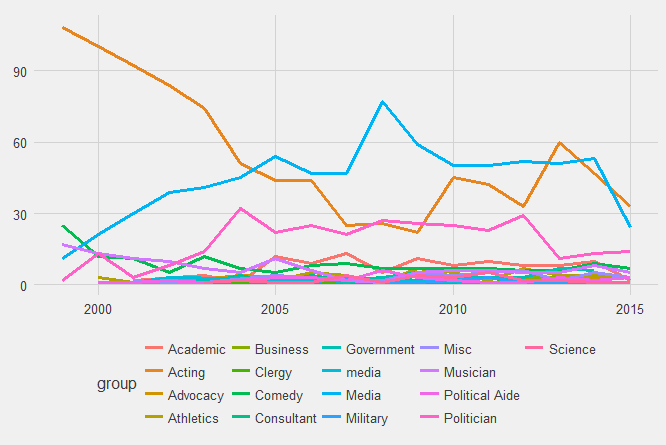
\includegraphics[width=.5\textwidth]{figures/dailyshow2}
		\label{Fig: 1}
		\end{figure}

%	\begin{verbatim}	
%
%dt <- daily\_show\_guests
%
%dt <- dt[!is.na(df\$group),]
%
%dt <- dt  \%>\% group\_by(year,group) \%>\% summarise(count = n())
%ggplot(df,  aes(x=year, y=count, colour=group)) + geom\_line() +  
%  theme\_fivethirtyeight()
%	\end{verbatim}




%	\begin{myexc}[Census data]
%	\fontsize{9pt}{11}\selectfont
%		\begin{enumerate}[(a)]
%			\item
%			Using the county data that you read into R earlier, produce a histogram, fixing the range of the x-axis to be $[0,70000]$ and the title to be something other than the default "Histogram of x" (\ul{Hint}: look at the documentation for \textts{\scriptsize hist()} options). Then, add a red vertical line at the location of the sample mean (\ul{Hint}: use \textts{\scriptsize abline()} and the option \textts{\scriptsize lwd} to make the vertical line more visible by changing its width). Finally, use \textts{\scriptsize density()} and \textts{\scriptsize lines()} to add an estimated density to the plot.
			
%				\begin{verbatim}


%ggplot(df, aes(value)) + 

%geom\_histogram(binwidth = 500, fill=I("blue")) + 

%ggtitle("County-level per capita income, 2013") +

%ylab("Count") +

%xlab("Value") +

%scale\_x\_continuous(labels = dollar) + \# install scales

%theme\_bw() +

%theme(plot.title = element\_text(size = 25, hjust = 0.5), 

%axis.title = element\_text(size = 20), 

%axis.text=element\_text(size=20)) 

%	\end{verbatim}
%		\end{enumerate}
%	\addtocounter{exccounter}{1}
%	\end{myexc}
	
%	\begin{figure}
%	\centering
%	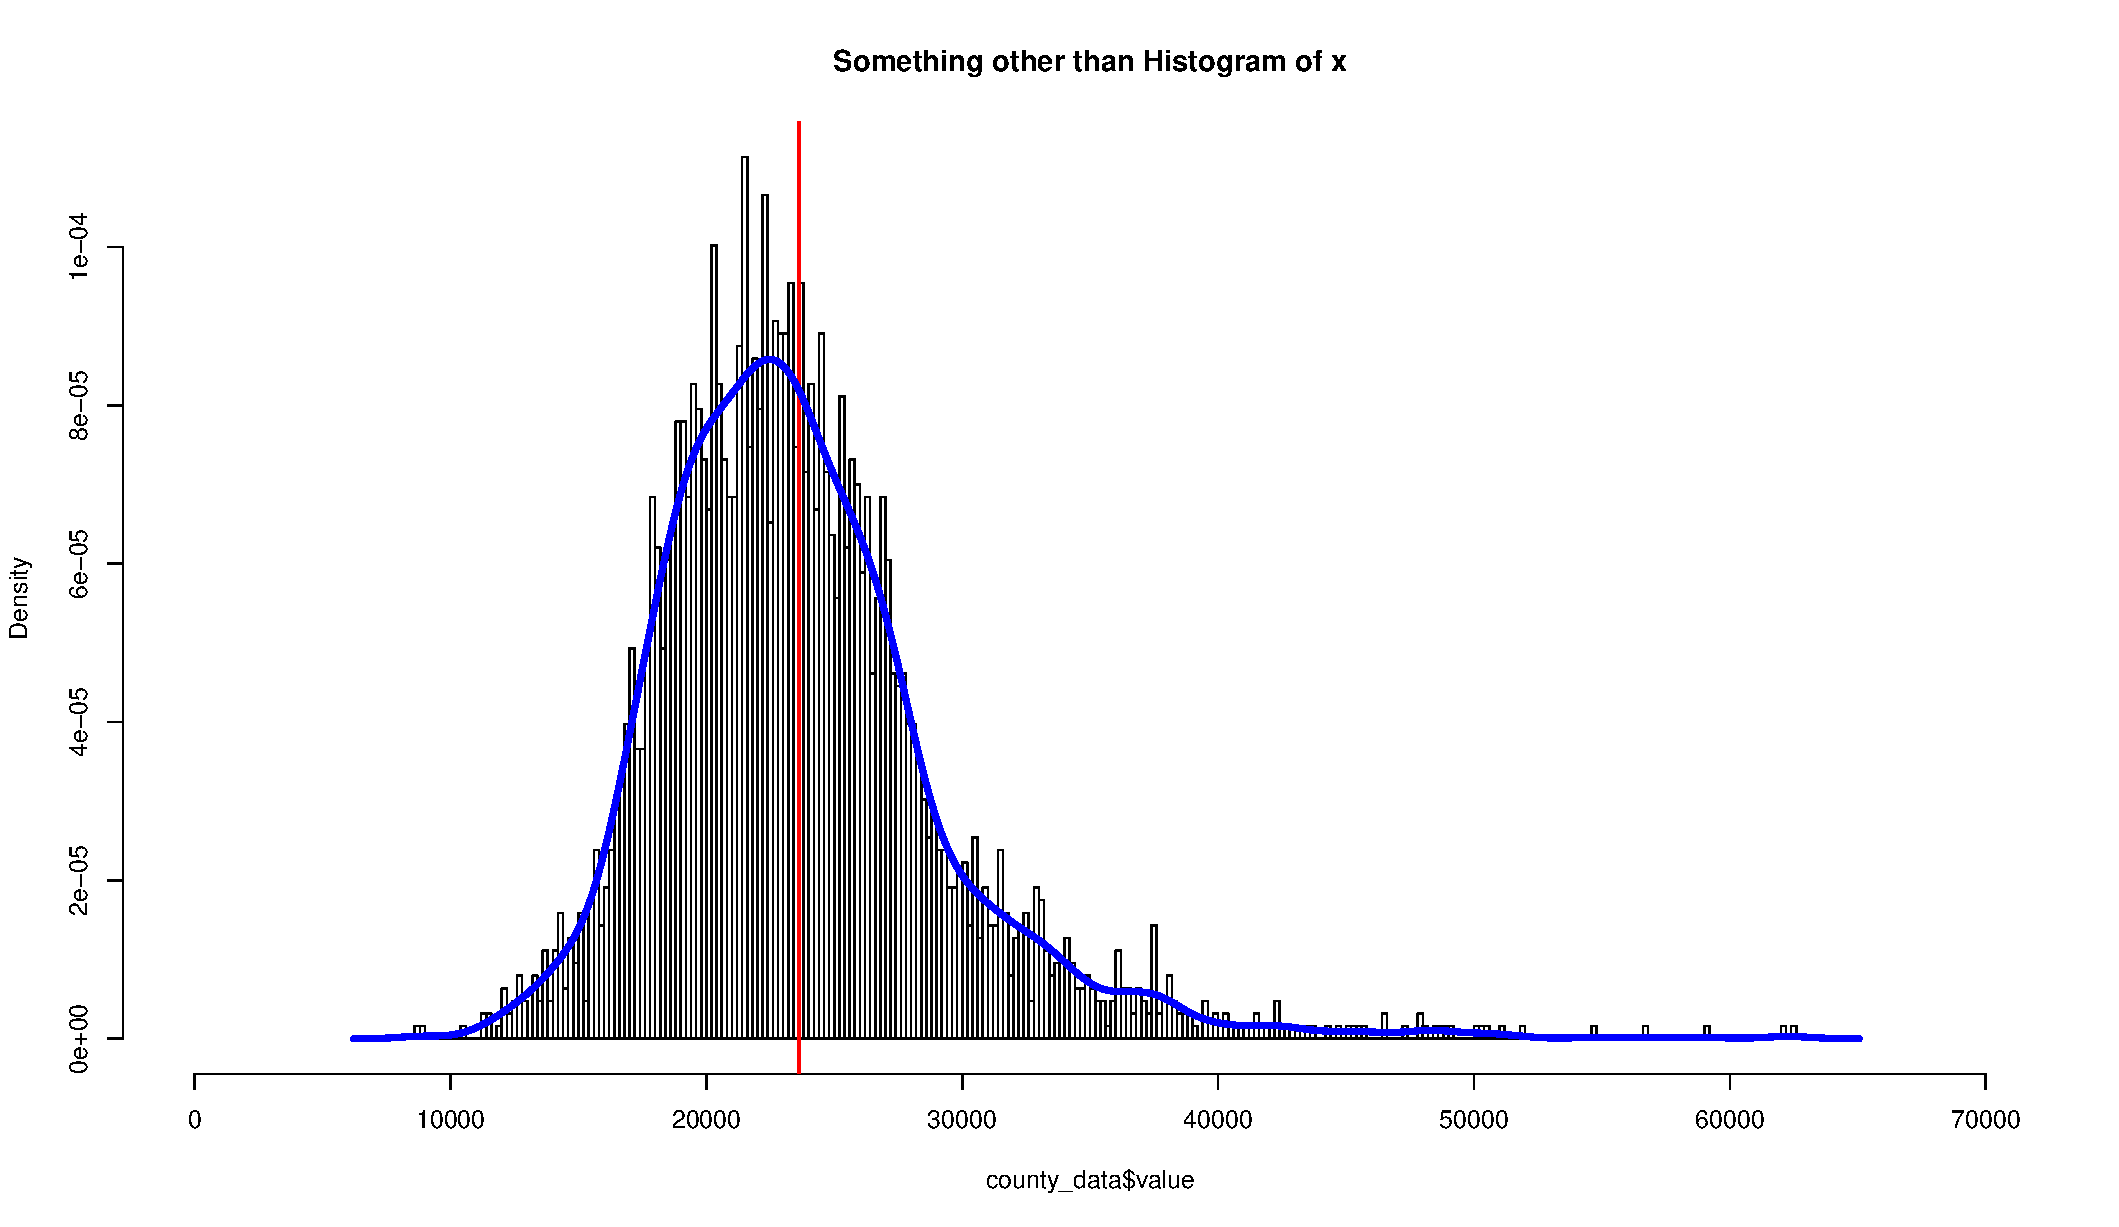
\includegraphics[width=0.7\textwidth]{figures/hist}
%	\caption{\scriptsize County per capita income.}
%	\label{Fig: hist}
%	\end{figure}
	




\end{frame}




\subsection{The \small\texttt{ggmap} \normalsize package}

\begin{frame}[allowframebreaks]
 \frametitle{The \Large\texttt{ggmap} package}
 
	\begin{itemize}
	    \item
	    We'll walk through an example of how to make maps with \textts{ggmap}.
	    \vfill
	    \item
	    Working with geospatial data is slightly more complicated than working with the data sets stored in .csv files that you are probably used to:
	    \begin{itemize}
	        \item
	        You need special data files that can tell R how to produce maps for the area you're interested in.
	        \item
	        These files are called \textbf{shape files}.
	        \vfill
	    \end{itemize}
	    \item
	    You can get shape files from the Census, or open data portals like the one provided by the city of Chicago: \scriptsize\url{https://data.cityofchicago.org/}\normalsize.
	    \vfill
	    \item
	    When you download shape files (e.g. myworld.shp), you will need to make sure you also have the DBF, Projection, and SHX files (e.g. myworld.dbf and myworld.prj and mywold.shx).
	    \begin{itemize}
	        \item
	        Make sure all the files have the same name (except for the extension) and are in the same directory.
        \end{itemize}
	\end{itemize}
	
	\begin{myexc}[Chicago grocery stores]
	\fontsize{9pt}{11}\selectfont
	We will plot the locations of Chicago grocery stores, and the community areas of Chicago.
		\begin{enumerate}[(a)]
			\item
			Load the following packages (remember you need to install them first if you have never used them before):\\
			\textts{library(rgdal) \# used to load the shapefiles}\\
            %\textts{library(dplyr) \# because I wouldn't leave home without it}\\
            \textts{library(ggmap) \# used to plot at the end}\\
            \textts{library(sp) \# should have been loaded as a required package of rgdal}
            \item
            Download a \textts{.csv} file with data on the location of grocery stores here: \scriptsize\url{https://data.cityofchicago.org/Community-Economic-Development/Grocery-Stores-2013/53t8-wyrc/data}\footnotesize. This is called ``point data''. It pinpoints the lat and long of all grocery stores. (You may learn more if you don't replicate my analysis exactly, maybe download \href{https://data.cityofchicago.org/Public-Safety/Crimes-2001-to-present-Dashboard/5cd6-ry5g}{Chicago crime} or other data besides grocery stores.)
            \item
            Download shape files on the division of community areas in Chicago here: \scriptsize\url{https://data.cityofchicago.org/api/geospatial/cauq-8yn6?method=export&format=Shapefile}\footnotesize. This is the cookie cutter file that has the information to produce outlines of community areas. You will see that this is a zip file that contains all of the files outlined above. Extract all files in the zip file and save in the same folder as the grocery store data.
		\end{enumerate}
	%\addtocounter{exccounter}{1}
	\end{myexc}
	
	
	\begin{myexccont}[Chicago grocery stores, cont'd]
	\fontsize{9pt}{11}\selectfont
		\begin{enumerate}[(a)]
			\item[(d)]
			The point data we downloaded from the Chicago data portal is a .csv file. We can use ggmap to import a map (instead of supplying a shape file), and show the points representing the locations of grocery stores, using ggmap. First, set your working directory to the folder where you saved the grocery store data. Then:\\
			\textts{pointdf <- read\_csv(file="Grocery\_Stores\_-\_2013.csv") \# import data}\\
			\textts{chicago <- get\_map(location = "chicago", zoom = 11) \# import map}\\
            \textts{ggmap(chicago) + }\\
            \textts{geom\_point(data = pointdf, aes(x = LONGITUDE, y = LATITUDE)) +}\\
            \textts{ggtitle("Map of Chicago Grocery Stores")}
            %\item
            %You can add more features just like a normal ggplot.
		\end{enumerate}
	%\addtocounter{exccounter}{1}
	\end{myexccont}


	\begin{figure}
	\centering
	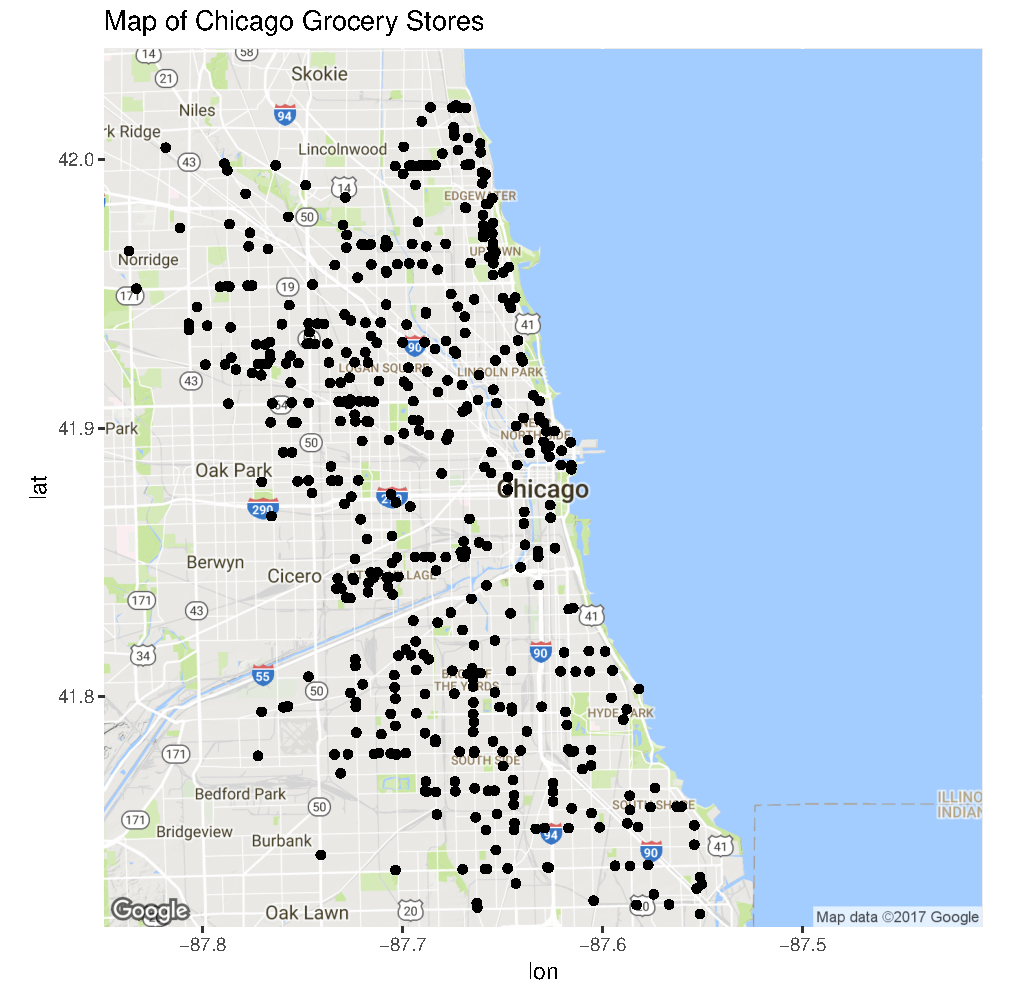
\includegraphics[width=0.6\textwidth]{figures/grocerystores}
	%\caption{\scriptsize County per capita income.}
	\label{Fig: map}
	\end{figure}
	
	
	\begin{myexccont}[ggmap, cont'd]
	\fontsize{9pt}{13}\selectfont
		\begin{enumerate}[(a)]
            \item[(e)]
			Set your working directory to the folder that holds the shape files. Then, plot the polygon file:\\ \tiny
            \textts{setwd("$\sim$/Desktop/BoundariesCommunityAreas")}\\
            \textts{overlay <- readOGR(".","geo\_export\_1490575f-394f-47c5-87b9-54097ef1b26f")}\\
            \textts{\# your file may have a different name}\\
            \textts{overlay <- spTransform(overlay, CRS("+proj=longlat +datum=WGS84"))}\\
            \textts{overlay <- fortify(overlay) %\# it works w/o this, but I figure you eventually want community names
            }\\
            \textts{location <- unlist(geocode('4135 S Morgan St, Chicago, IL 60609')) + c(0,.02)}\\
            \textts{gmap <- get\_map(location=location, zoom = 10, maptype = "terrain", source = "google", col="bw")}\\
            \textts{gg <- ggmap(gmap) + geom\_polygon(data=overlay, aes(x=long, y=lat, group=group), color="red", alpha=0)}\\
            \textts{gg}
		\end{enumerate}
	%\addtocounter{exccounter}{1}
	\end{myexccont}

    \vskip.5cm
    \scriptsize [Example based on \tiny\url{https://stackoverflow.com/questions/26344510/overlaying-polygons-on-ggplot-map}.]

	\begin{figure}
	\centering
	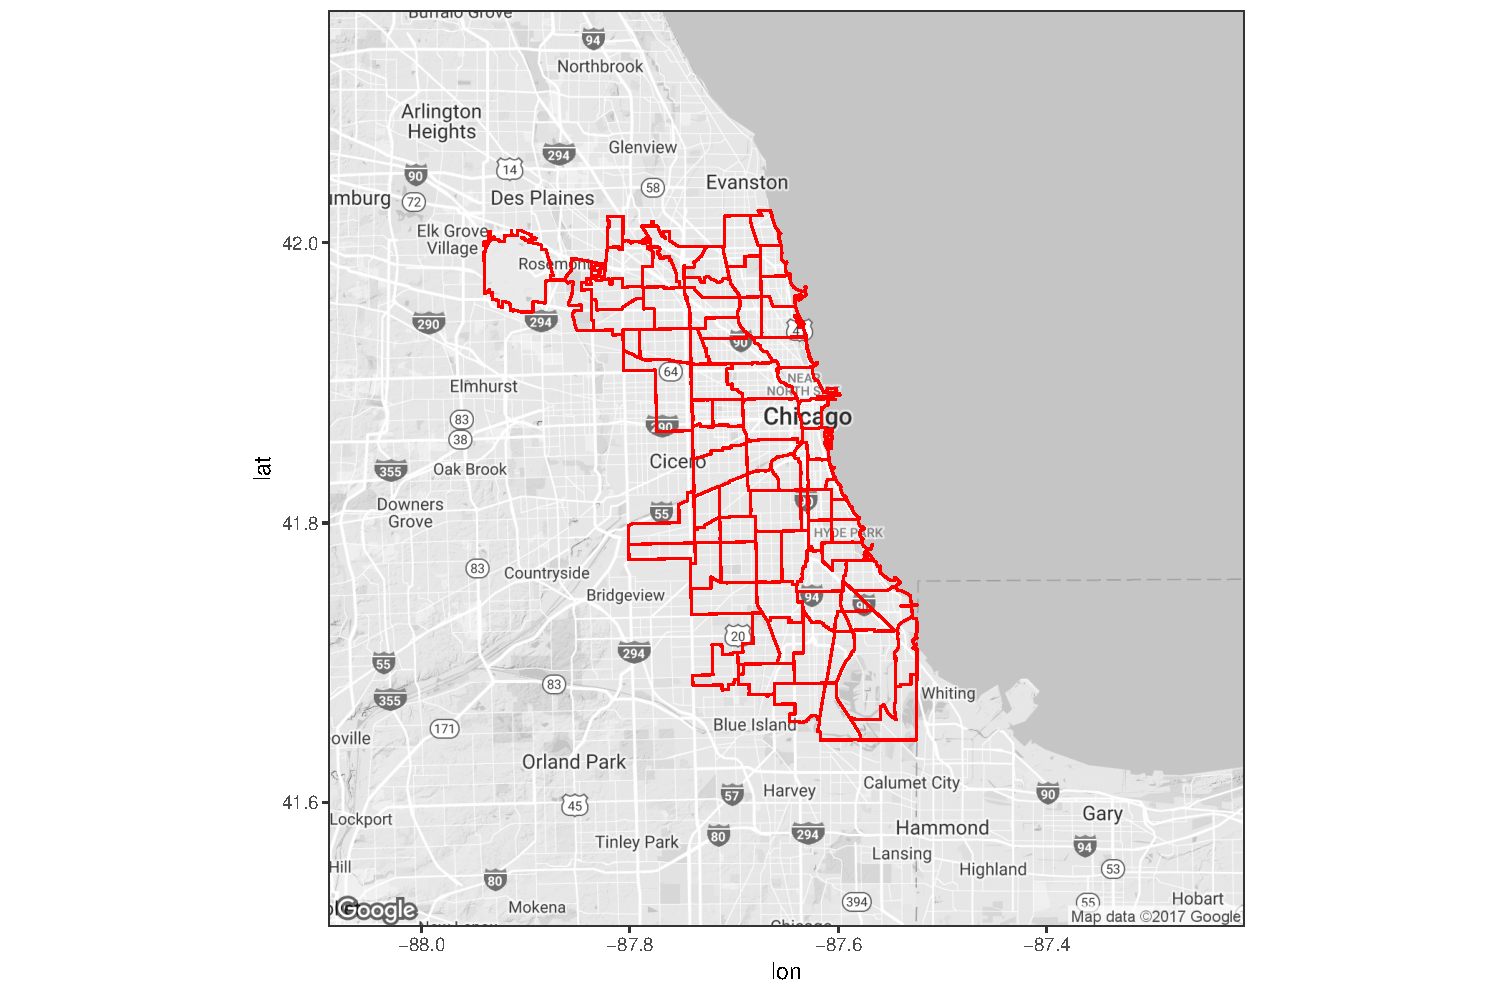
\includegraphics[width=0.9\textwidth]{figures/mapchicagocomm}
	%\caption{\scriptsize County per capita income.}
	\label{Fig: map}
	\end{figure}
	
	
	\begin{myexccont}[ggmap, cont'd]
	\fontsize{9pt}{11}\selectfont
		\begin{enumerate}[(a)]
            \item[(f)]
			Create a map with community areas as in (e), overlaying the locations of grocery stores as in (d).
		\end{enumerate}
	%\addtocounter{exccounter}{1}
	\end{myexccont}

	\begin{figure}
	\centering
	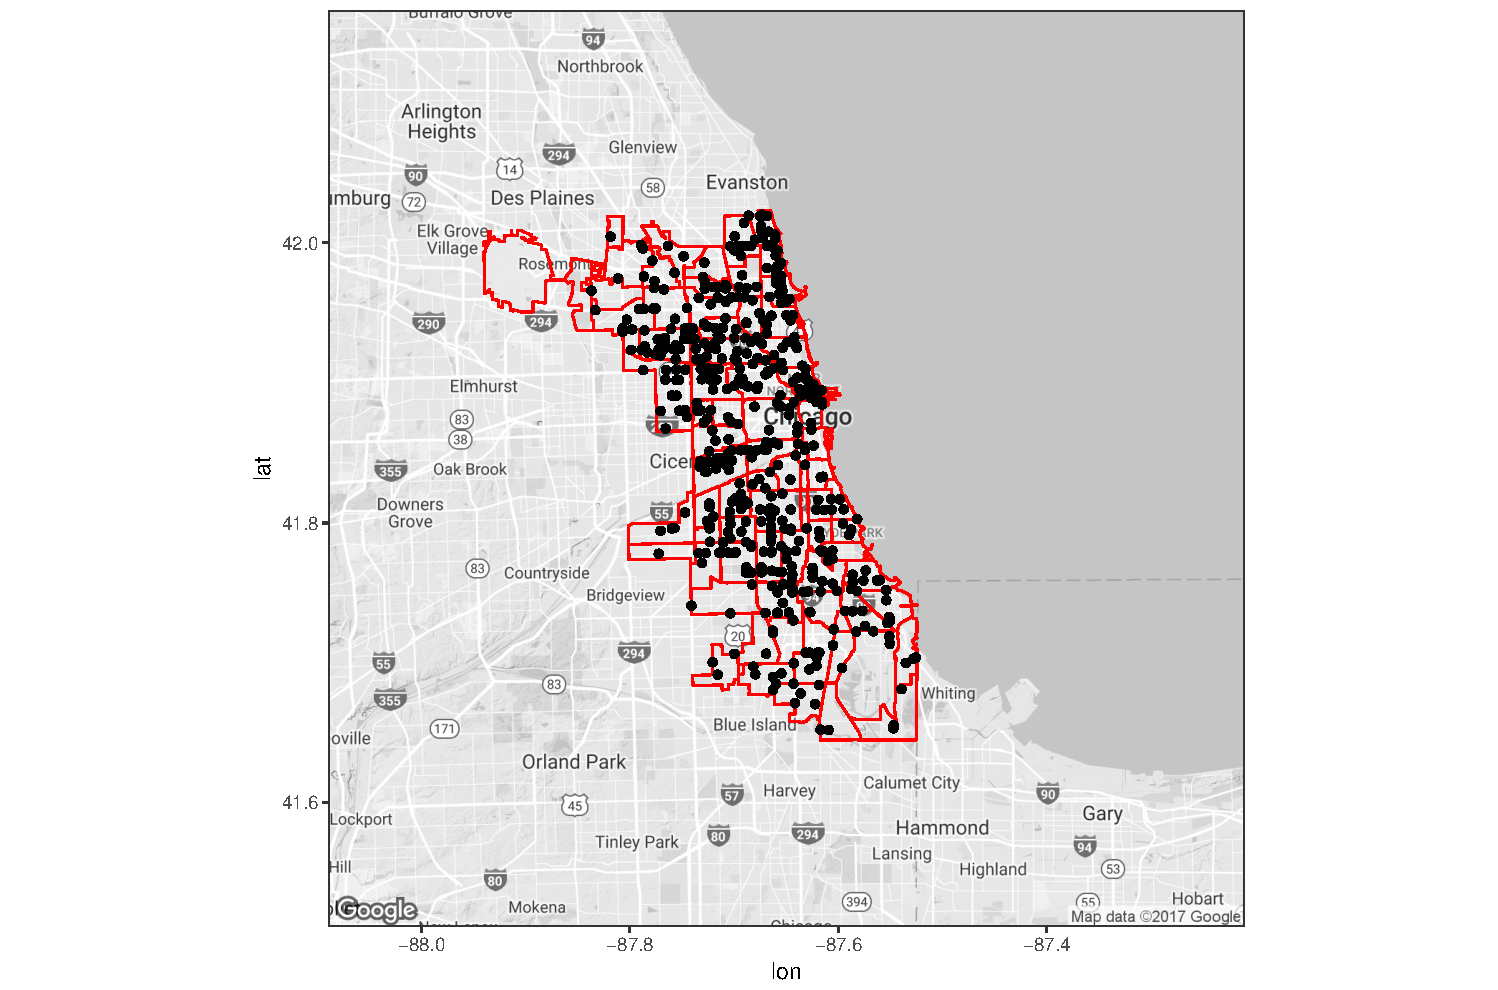
\includegraphics[width=0.65\textwidth]{figures/grocerystores2}
	%\caption{\scriptsize County per capita income.}
	\label{Fig: map}
	\end{figure}
	
	\begin{myexccont}[ggmap, cont'd]
	\fontsize{9pt}{11}\selectfont
		\begin{enumerate}[(a)]
            \item[(g)]
			Create a map with community areas as in (e), but with the areas shaded according to the number of grocery stores in that area.
		\end{enumerate}
	%\addtocounter{exccounter}{1}
	\end{myexccont}

	\begin{figure}
	\centering
	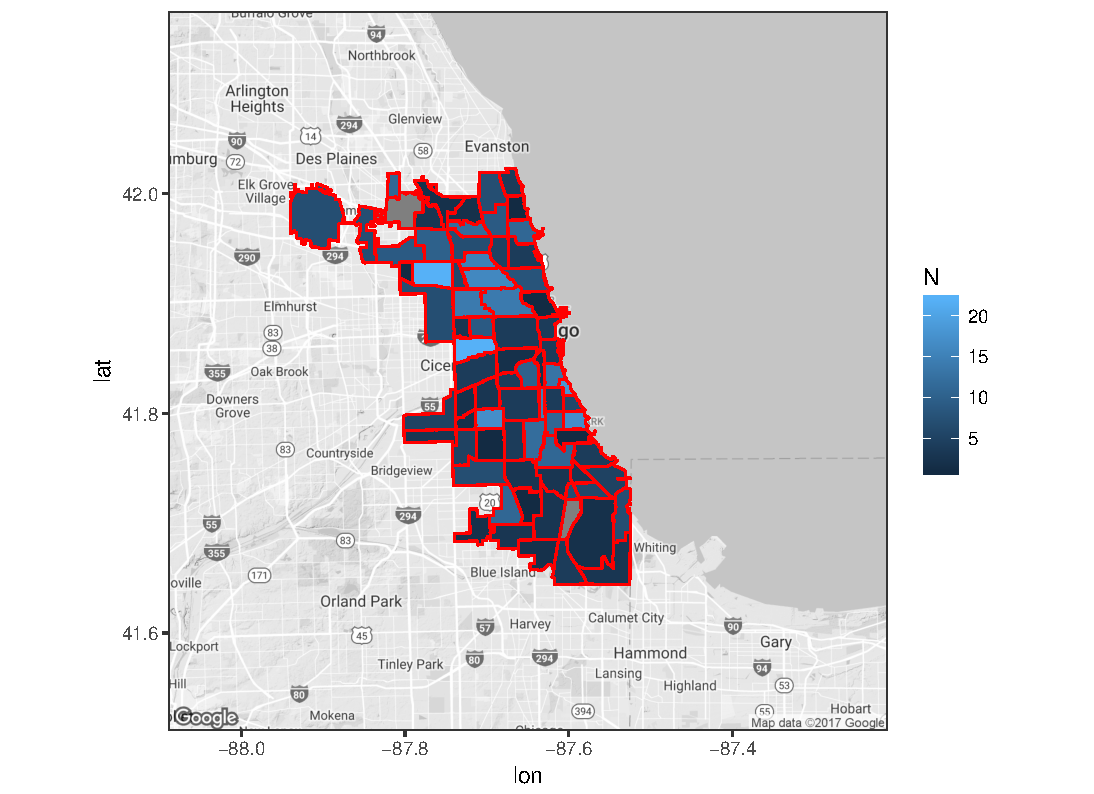
\includegraphics[width=0.6\textwidth]{figures/Grocery_shaded_areas}
	%\caption{\scriptsize County per capita income.}
	\label{Fig: map}
	\end{figure}
	
	%\vskip-.6cm
	\footnotesize
	Code used in part (g):\tiny
	\begin{verbatim}
	
pointdt <- data.table(pointdf) \# convert to data.table for convenience


ca\_storecount <- pointdt[, .(.N), by = `COMMUNITY AREA`] \# count number of stores per community area


overlay <- readOGR(".","geo\_export\_a3feb55a-afb1-4aca-839e-6882c81c8c08") \# your file may have a different name


overlaydata <- data.table(overlay@data) \# extract the data part


overlaydata <- merge(overlaydata, ca\_storecount, by.x = "area\_numbe", by.y = "COMMUNITY AREA", all.x = TRUE, all.y = FALSE) \# merge in the store counts


overlaydata\$id <- sapply(slot(overlay, "polygons"), function(x) slot(x, "ID")) \# add ids that correspond to the slot ids in overlay


overlay <- data.table(fortify(overlay))


overlay <- merge(overlay, overlaydata, by = 'id') \# merge the data back in


gmap <- get\_map(location = location, zoom = 10, maptype = "terrain", source = "google", col = "bw")


gg <- ggmap(gmap) + geom\_polygon(data = overlay, aes(x = long, y = lat, group = group, fill = N), color = "red", alpha = 1)

	\end{verbatim}	

	\begin{myexccont}[ggmap, cont'd]
	\fontsize{9pt}{11}\selectfont
		\begin{enumerate}[(a)]
            \item[(h)]
			Change the color scheme: \textts{gg + scale\_fill\_gradient(low = 'grey', high = 'red')}.
		\end{enumerate}
	\addtocounter{exccounter}{1}
	\end{myexccont}

	\begin{figure}
	\centering
	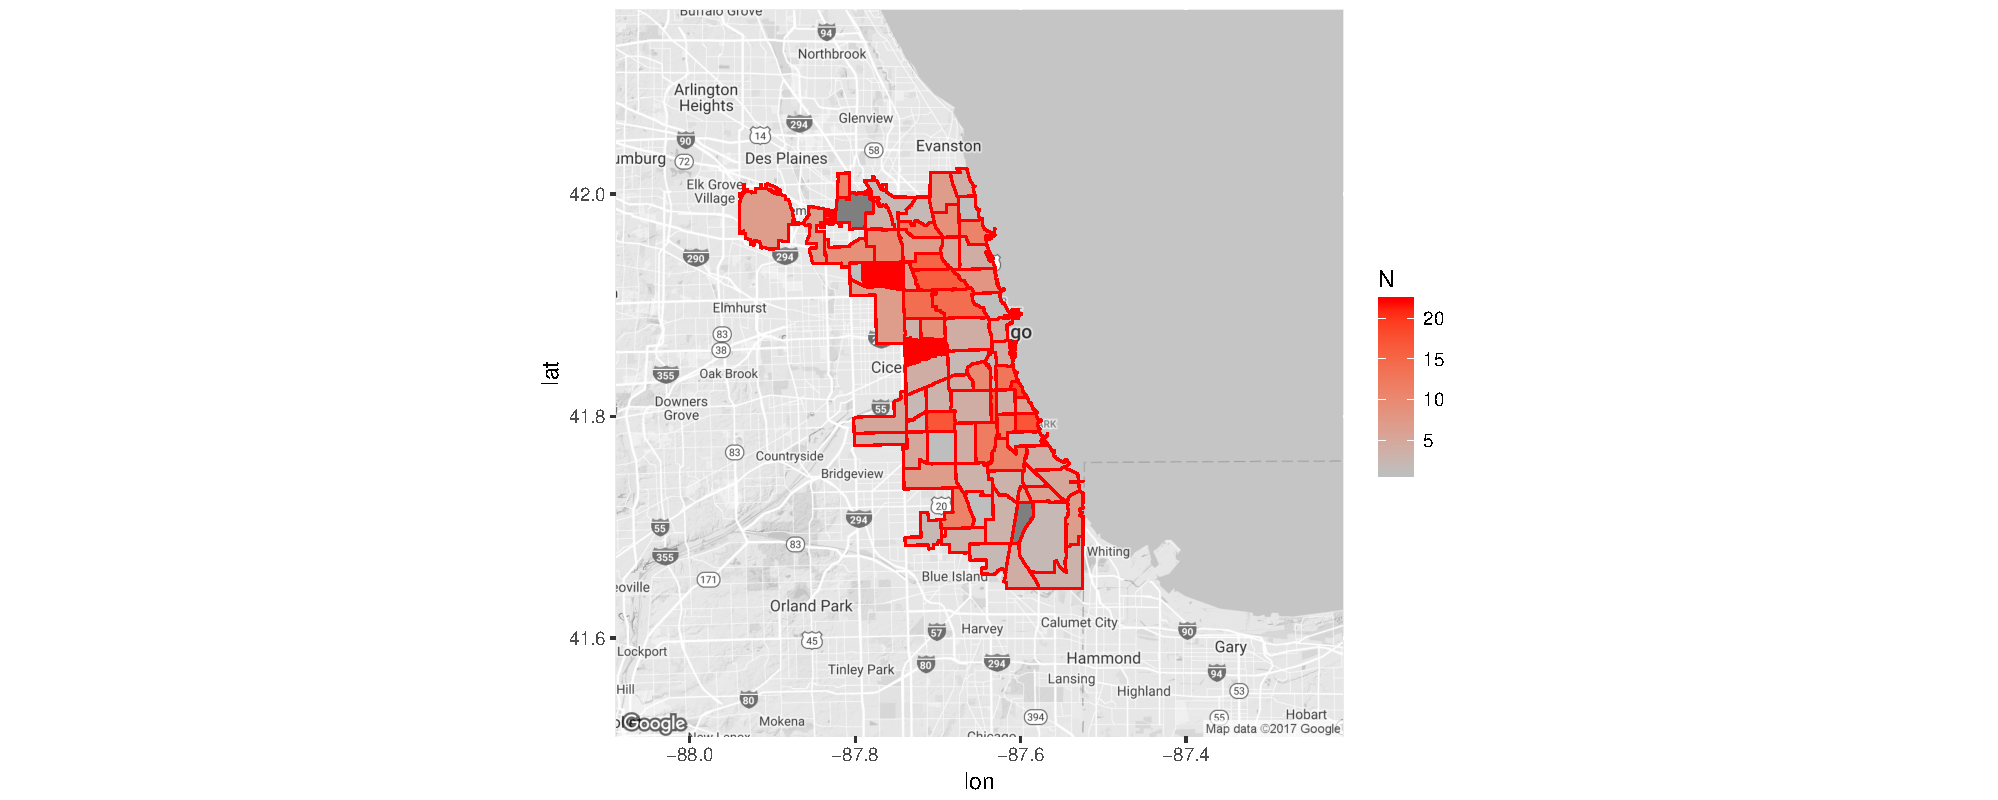
\includegraphics[width=1.1\textwidth]{figures/Grocer_stores_shaded2}
	%\caption{\scriptsize County per capita income.}
	\label{Fig: map}
	\end{figure}
	


\end{frame}






\section{Reporting}

\begin{frame}[allowframebreaks]
 \frametitle{}
 
    There are several options available for reporting on your R output, including:
    \vskip.5cm
    \begin{itemize}
	    \item
	    R Notebooks
        \vskip.5cm
	    \item
	    Shiny
        \vskip.5cm
	    \item
	    Knitr
        \vskip.5cm
	    \item
	    Jupyter notebooks
	\end{itemize}
	
\end{frame}










\section{Some useful packages}

\begin{frame}[allowframebreaks]
 \frametitle{Packages}
    
    A couple of packages you may find useful:
	\begin{itemize}
        \item
        \textts{AER}: Data sets used for examples in several textbooks
        \item
        \textts{psidR}: Creating data sets from PSID data
        \item
        \textts{Rcpp}: Integrate C++ code to speed up computation
        \item
        \textts{RColorBrewer}: Make custom color schemes for plotting
        \item
        \textts{parallel}: Parallel processing in R, will help you speed up computation
        \item
        \textts{zoo}: for working with time series
	    \item
	    \textts{wru}: Bayesian prediction of racial category using surname and geolocation
	\end{itemize}
	
	%\vskip.5cm
	
	You can also build your own packages, to bundle functions and documentation built to perform specific tasks, or just to collect your own auxiliary functions that you often use. Here are some guidelines: \scriptsize\url{http://r-pkgs.had.co.nz/}\normalsize.
	
	\vskip10cm
	
	The R packages ecosystem:
		\begin{figure}
		\centering
		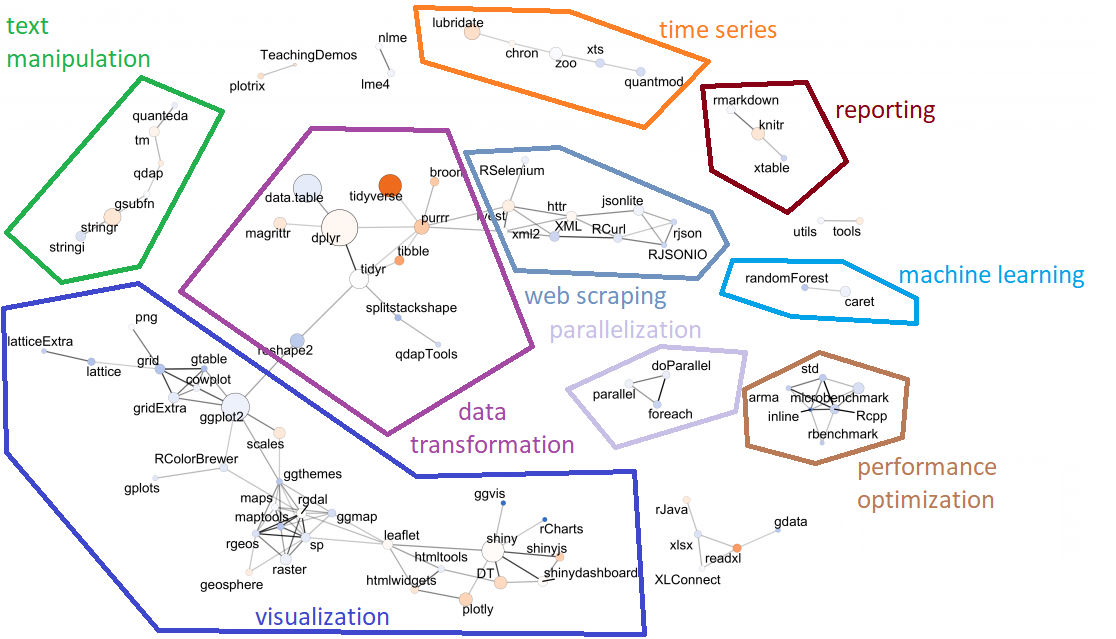
\includegraphics[width=.8\textwidth]{figures/rpackages_eco_cat}
		\caption{\scriptsize The `Ecosystem of R packages': correlations are based on packages mentioned in Stack Overflow answers on the same question. This image is taken from \tiny\url{https://stackoverflow.blog/2017/10/10/impressive-growth-r}\scriptsize.}
		\label{Fig: 1}
		\end{figure}
	
\end{frame}






%\subsection{Building your own package}
%
%\begin{frame}[allowframebreaks]
% \frametitle{Building your own package}
% 
%    \begin{itemize}
%	    \item
%	    ...
%	\end{itemize}
%	
%\end{frame}




























\section{Recommended resources}

\begin{frame}[allowframebreaks]
 \frametitle{Recommended resources}

 \textbf{R:}
 \begin{thebibliography}{10}

 \beamertemplatebookbibitems
 
 \bibitem{RIntroCore}
 W.N. Venables, D.M. Smith and the R Core Team - An Introduction to R
 \newblock{}
 \newblock{2017 version}
 \newblock{\scriptsize \url{http://cran.r-project.org/doc/manuals/R-intro.pdf}}

% \bibitem{StockWatson}
% J.H.~Stock \& M.W. Watson (3rd ed)
% \newblock {\em Introduction to Econometrics: Chapter 1, Sections 2.1-2.4, and Appendices 17.1, 17.2, 18.2.}

 \beamertemplateonlinebibitems
 
 \bibitem{RStudioTips}
 RStudio: Tips for learning R
 %\newblock{\em }
 \newblock{\scriptsize \url{http://www.rstudio.com/online-learning/}}
 
 \bibitem{GoogleRStyle}
 Google's R Style Guide
 %\newblock{\em }
 \newblock{\scriptsize \url{https://google.github.io/styleguide/Rguide.xml}}
 
 \bibitem{tryr}
 TryR
 \newblock{}
 \newblock{Online interactive tutorial for first steps in R}
 \newblock{\scriptsize \url{http://tryr.codeschool.com/}}
 
 \bibitem{Forums}
 Stack Overflow, Cross Validated
 \newblock{}
 \newblock{Forums for programming and statistics questions}
 \newblock{\scriptsize \url{http://stackoverflow.com/}} and {\scriptsize \url{http://stats.stackexchange.com/}}
 
 \bibitem{MacR}
 Google Developers' Intro to R
 \newblock{}
 \newblock{Youtube tutorial videos -- geared towards Mac users}
 \newblock{\scriptsize \url{http://www.youtube.com/playlist?list=PLOU2XLYxmsIK9qQfztXeybpHvru-TrqAP}}
 
 \bibitem{HW}
 Hadley Wickham - Advanced R
 \newblock{}
 \newblock{Companion website for Advanced R book}
 \newblock{\scriptsize \url{http://adv-r.had.co.nz/}}
 
 \bibitem{GGHW}
 Garrett Grolemund \& Hadley Wickham - R for Data Science
 \newblock{}
 \newblock{Companion website for R for Data Science book}
 \newblock{\scriptsize \url{http://r4ds.had.co.nz/}}
 
 \bibitem{TS}
 Tom Short - R Reference Card
 \newblock{}
 \newblock{A useful cheat sheet, though somewhat outdated}
 \newblock{\scriptsize \url{http://cran.r-project.org/doc/contrib/Short-refcard.pdf}}
 
 \bibitem{TS}
 Knitr page, by Yihui Xie
 \newblock{}
 \newblock{Instructions for installing and using Knitr, a tool for integrating R code into LaTeX documents}
 \newblock{\scriptsize \url{http://yihui.name/knitr/}}

 \end{thebibliography}

\end{frame}



\end{document}